\begin{figure*}[!ht]
\centerline{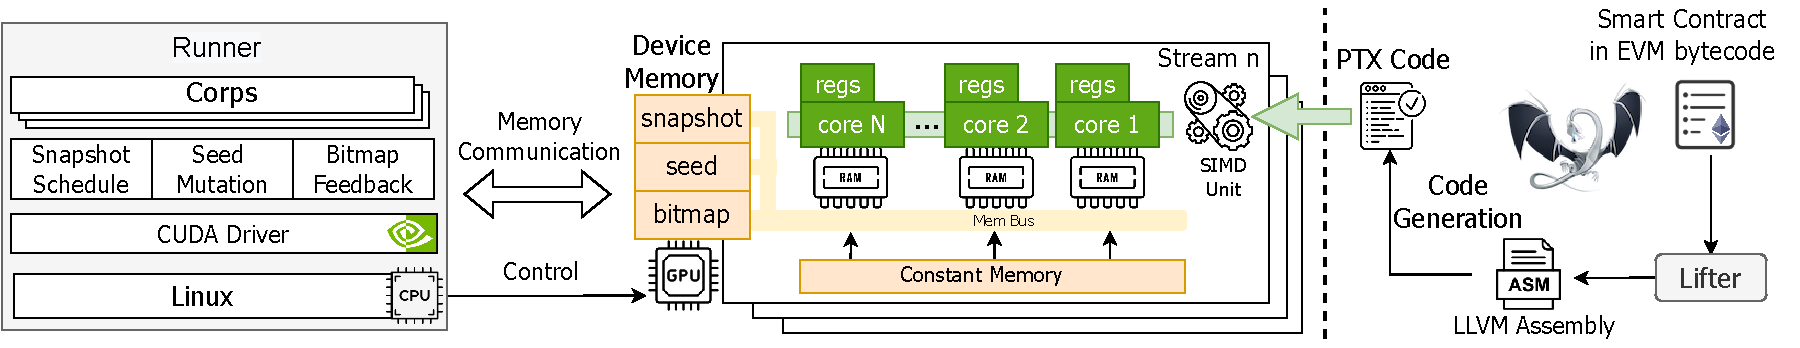
\includegraphics[width=\textwidth]{images/GFL-overview.drawio.pdf}}
\caption{The overview of {\tool}. {\translator} first translates the given bytecode to a PTX code which GPU can load for parallel fuzzing under the guidance of {\runner}. {\translator} only executes once for each fuzzing application.}
\vspace{-0.1in}
\label{fig:overview}
\end{figure*}

\section{Design}
\label{sec:design}

Figure~\ref{fig:overview} depicts the architecture of the {\tool}, which parallelly tests a smart contract using the GPU SIMD architecture.
% Based on binary translation technology, {\tool} can fuzz the smart contract even if its source code is unavailable.
%
GPU can load a PTX code which the SIMD unit dispatches to every GPU thread (See Figure~\ref{fig:overview}(c)). 
We define $i$ as the thread ID, which GPU uses to label the parallel thread.
In each moment, all running threads execute the same PTX instruction together but obtain different seeds via data parallelism\cite{cuda2006datapara}.
For example, all seeds are encoded to global data in GPU, where thread $i$ can compute the address of its seed using its thread ID.
%
%
To be specific, the process pipeline of {\tool} consists of five steps. 
%
First, given an EVM bytecode, {\translator} translates it into a functional equivalent LLVM assembly, where the opcodes for EVM components (e.g., stack, memory and storage) are abstracted in LLVM memory operations.
%
Second, {\translator} rewrites the memory operations of the LLVM assembly from the on-the-fly translation, enabling the fuzzing threads to be free of branches via data parallelism.
% Second, {\wrapper} creates a GPU kernel function in LLVM IR to wrap the contract code from {\translator}, for the parallel execution in GPU. The kernel function schedules graphic memory for thousands of GPU threads, allowing all threads to execute independently with different inputs. The wrapped LLVM assembly will be translated into a PTX executable as the final fuzzing target. 
%
The third step is code generation producing a PTX smart contract from the established LLVM assembly using the LLVM backend\cite{llvm2021bin}.
Next, {\runner} generates seeds and executes them with the PTX smart contract in thousands of threads. 
{\runner} is also equipped with snapshot strategies and coverage-based feedback to guide the seed mutation.
At last, {\runner} mutates seeds and repeats the fourth step until any bugs are detected. 
%


This section introduces {\runner} and then {\translator}.
The first part presents the targets of fuzzing a smart contract on GPU.
The second part explains the design choices of {\translator} in generating a smart contract equipped with the components required by {\runner}.


\subsection{{\runner}: High Performance Fuzzing}
Throughput indicates the number of seeds that fuzzers can test in a unit of time.
%
The execution speed of the target program is one fundamental factor in fuzzing throughput\cite{fuzzan_atc}. 
%
The existing work\cite{confuzzius_eurosp,echidna_issta} applies task parallelism to test multiple seeds together, where several processes run the smart contract independently in a multi-core machine.
%
However, the smart contracts are executed in an interpreted language (e.g., EVM bytecode\cite{wood2014ethereum}).
Official blockchain runtime (i.e., EVM) compromises performance for deterministic execution, which will bring too much overhead for fuzzing.
%
Although another potential attempt is to translate the EVM bytecode to CPU native code via JIT (just-in-time) compilation\cite{jit1998survey}, the JIT-fuzzers still share the same throughput bottlenecks with the classical fuzzers like AFL\cite{afl} and Angora\cite{angora_sp}. 
For example, the maximum number of parallel fuzzers cannot exceed 128 because of the hardware limit.
%
% Unfortunately, they still share the same throughput bottlenecks with the classical fuzzers like AFL\cite{afl} and Angora\cite{angora_sp}. 
% For example, the maximum number of parallel fuzzers cannot exceed 128 because of the limited CPU cores.
%
Therefore, in terms of fundamental aspects, existing fuzzing technologies cannot achieve the expected throughput in testing smart contracts (See \S~\ref{rq:throughput} for more details).


We believe the key of improving fuzzing throughput is running as many parallel threads as possible to test the smart contract 
%
Fuzzing is an ideal workload for parallel execution because all fuzzing threads are naturally free of lock.
To be specific, in each fuzzing thread, we can run the target smart contract independently with its own context, i.e., stack, memory and registers. 
The only synchronization event is used to wait for the end of all fuzzing threads so that the collected coverage information can guide the fuzzer to mutate new seeds.
%
The more threads we can schedule, the higher throughput the fuzzer can achieve.
That is the reason why we choose to fuzz smart contracts on GPU. 
Different from the CPU, GPU can run thousands of threads in parallel within its stream processors. 
%
One of the most powerful CPUs, AMD EPYC 9654(\$11,805), has 96 cores, but one single NVIDIA RTX3090 (\$999) can provide 10,496 CUDA cores\footnote{The prices come from the official vendor websites.}. 
The incredible computation power of GPU is attractive for parallel fuzzing because it is available to translate a smart contract to a GPU executable, i.e., PTX\cite{ptx2021doc}. 
%
Since GPU is based on SIMD architecture, we need to apply data parallelism rather than task parallelism.
%


% Running on CPU, {\runner} will launch a GPU device and fuzz the smart contracts with a batch of seeds together. Once the GPU jobs are finished, {\runner} obtains the coverage information to guide the seed generations. 

% In this section, we mainly elaborate the design and reasons of {\runner}, including SIMD execution for parallel fuzzing, snapshot strategy for handing transaction dependency (TBD).
%
% These strategies raise functional requirements to the smart contract and they can explain the design choices of the bytecode translation in \S~\ref{design:translator}.





\subsubsection{Asynchronous GPU Calls}

\begin{figure}[t]
\centerline{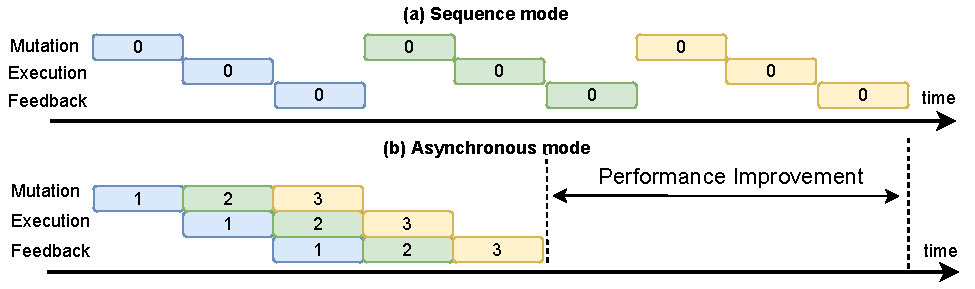
\includegraphics[width=0.5\textwidth]{images/GFL-async_cpy.drawio.pdf}}
\caption{Fuzzing Timelines}
\vspace{-0.1in}
\label{fig:async_cpy}
\end{figure}

To the best of our knowledge, classical fuzzers are implemented on the CPU. 
Their fuzzing steps are required to be executed sequentially.
On the one hand, the target application cannot run until the mutated seeds are prepared. 
On the other hand, the feedback has to run after the target application execution. 
%
Since GPU and CPU are two independent devices, {\runner} can reduce the time intervals between fuzzing tasks via asynchronous execution.
{\runner} invokes a GPU to execute the smart contract and immediately uses the CPU to run the fuzzing tasks.
%
The entire fuzzing workload is divided into several asynchronous streams.
Each stream consists of three kinds of tasks such as seeds mutation, smart contract execution, and bitmaps feedback. 
The threads in the same stream will run in parallel, but different streams run asynchronously. 
By executing a portion of the workload together, the fuzzing throughput can be improved. 
%
In Figure~\ref{fig:async_cpy}, we show the timelines for (a) sequential mode and (b) asynchronous mode. 
Three stream pipelines are used to handle the three groups of fuzzing tasks in asynchronous mode. 
The jobs in the same stream are highlighted in the same color. 
In the first time slot, we mutate seeds on the CPU only. 
In the next slot, stream $D_1$ and $D_2$ run together, which executes the smart contract on GPU and mutates seeds on the CPU, respectively. 
%
At last, we can finish the fuzzing work within five units of time, which is less than the classical approaches (nine units of time).
%
% Moreover, the asynchronous mode enables {\tool} to reduce the delay of memory latency. \cite{} analyzes the CUDA overhead and finds transferring data between CPU and GPU is time-consuming. {\tool} can invoke another streams when the memory bus of GPU is stuck to one stream job. 

% That is the reason why SIMD code should reduce branch divergence\cite{branchdiver2011gpgpu} to improve performance.
%

\begin{figure}[ht]
    \centering
    \lstinputlisting[language=Solidity,linewidth={\linewidth},frame=tb,basicstyle=\footnotesize\ttfamily]{code/tx_dep.sol}
    \vspace{-0.1in}
    \caption{An Example for Transaction Dependency.}
    \label{fig:code_tx_dep}
\end{figure}

\subsubsection{Snapshot Schedule}
\label{design:snapshot}
The smart contract is a stateful program that maintains state variables in its storage. Since state variables can be a part of branch conditions, some branches can only be explored by fuzzers when the smart contract storage is set to specific content. 
We call this hurdle as transaction dependency (\textbf{C2}).
%
Figure~\ref{fig:code_tx_dep} shows an example where the integer underflow bug in function $vul()$ can only be triggered when the state variable named $locked$ is set to \texttt{false} via executing $dep(false)$ before. 
%
To handle the transaction dependency, existing fuzzers generate a sequence of transactions as one seed\cite{confuzzius_eurosp, echidna_issta, ilf_ccs}. 
%
% To be specific, they first choose one transaction and then combined it with other transactions to generate a sequence-based seed. 
%
However, they may execute duplicated transactions, resulting in fuzzing overhead. 
For example, all useful seeds must share the same first transaction, i.e., $dep(false)$ and then mutate the input of $vul()$ to construct the second transaction.
To shave off common prefixes from the execution, {\tool} takes an incremental snapshot of the storage after the common transactions were executed.
%
% To address this issue, we design storage snapshots to switch fuzzing states. 
% An interesting seed can explore new branches of the smart contract. 
% After testing the interesting seed, we export the finalized content of the storage as an interesting state.
%

Each snapshot is a byte string representing the storage content. 
{\tool} starts each new execution from the root snapshot that represents an initial state, i.e., real-world storage.
{\tool} can create a new snapshot just after executing one given transaction, marking a check point. 
By reloading the snapshot, we rollback the smart contract and test it a number of times with different seeds.
% i.e., the storage updated by $vul()$ in Figure~\ref{fig:code_tx_dep}.
%
% {\tool} can 
%
By switching snapshots, {\tool} can handle the transaction dependency without using transaction duplication. 


%
The storage data originally associated with the root snapshot remains in place; the new ones are written to an incremental snapshot\cite{row2021ibm}.
%
This design is based on our observation that one transaction usually only modifies a few storage data. 
%
Here are some details.
Before launching the GPU threads, we load a storage snapshot as the root snapshot $m$, which is a read-only array exposing to all threads.
$N$ is a vector representing the storage snapshot for all threads, where $N_i$ indicates the incremental snapshot of the storage used by thread $i$.
%


\subsubsection{Coverage Feedback}
\label{sec:runner:coverage}
{\runner} records the coverage information to a bitmap.
The bitmap is a serial array where the compile-time inserted instructions will update the bitmap when the smart contract is running. 
%
The bitmap content should contain both the explored edges and changes of the state variable to guide the stateful fuzzing.


The feedback of the traditional coverage-based fuzzers is based on the explored branches.
For example, AFL uses a tuple $(src, dst)$ to record an explored edge, i.e., a control flow from one basic block to another one. Whenever a basic block is executed, the bitmap byte in the index of $src \ll 1 \oplus dst$ increases by one. 
Since smart contracts are stateful, we extend the bitmap to reflect the changes in the state variables. 
To be specific, the bitmap index of the explored edge is a hash value from the coverage information: 
$$
hash(src,dst,states) = state_0 ... \oplus state_n \oplus src \ll 1 \oplus dst
$$ , where $state_i$ indicates one storage variable. (TBD)


Inspired by AFL\cite{afl}, we encode the coverage of each thread to an array named
\texttt{virgin\_bits}\cite{afl}, denoted as $b$. 
It is helpful for {\runner} to faster counter new bits from a bitmap.
\texttt{virgin\_bits} has the same size as a bitmap.
Each byte (i.e., $b_j$) represents whether the corresponding branch is touched or not.
Initially, the entire \texttt{virgin\_bits} is fully masked, i.e., each byte value is 0xff.
We set $b_j$ to zero if there exists one bitmap touching the branch $j = hash(src,dst,states)$. 
If $b_j$ remains 0xff, {\runner} considers the branch has not yet been explored by any seeds. 

\subsubsection{Seeds Mutation}
\label{design:mutation}
We create a sequence of bytes in the GPU memory to maintain the seeds vector for all fuzzing threads, denoted as $S$.  
$S_{ij}$ indicates the $j$ byte of the seed used by the thread $i$.  
Each seed is padded to a fixed size for threads to access it with a runtime offset.
If $S_i$ is interesting, {\runner} will mutate it to generate more seeds. 
Each seed is a byte array consisting of three parts such as \texttt{calldata}, \texttt{calldatasize} and \texttt{callvalue}, representing the input of smart contract, the size of \texttt{calldata} and the amount of cryptocurrency (i.e., Ether), respectively.  
%
The first fourth bytes of \texttt{calldata} represent a function signature, and its following bytes are its function arguments serialized based on the ABI\cite{abi}.
ABI (Application Binary Interface) describes the headers of the smart contract functions, such as signatures and argument types. 
It is usually public along with smart contract bytecode.
%
Thanks to the parallel fuzzing, {\runner} is able to test all functions with thousands of threads. 
In the beginning, we establish the fourth bytes of each seed as one function signature and then generate initial bytes as the function arguments.
During the fuzzing, {\runner} focuses on mutating the arguments bytes based on the ABI.
% The sequence of bytes belonging to the same function argument should be mutated together.
%
% In \S~\ref{}, we have leveraged snapshot mechanism to select the tested function of a smart contract. 
%
% In this part, we focus on mutating the function arguments. Specifically, we mutate the calldata starting from the fourth byte. 
%
% As calldata is constructed following the ABI grammar, some sequence of bytes belong to the same function argument. Thus, they should be mutated together.
%
% To this end, we parse the ABI and then identify the affine types between the raw calldata bytes and high-level function arguments. 
%
According to the function headers recorded in ABI, we mutate the bytes according to the types of the function arguments. 
For each byte sequence, we mutate them using AFL\cite{afl} approaches such as bit flipping, bytes walking and so on.
Note that we update \texttt{calldatasize} for the new seed. \texttt{callvalue} is set to a large constant, assuming we have enough cryptocurrency. 

Apart from seeds, {\runner} also provides some configures for the testing smart contract, such as  \texttt{tx.sender} and \texttt{tx.origin}, representing the account address of the transaction sender and the original sender, respectively. 
We assume {\tool} has the owner privilege to test the smart contract. Thus both \texttt{msg.caller} and \texttt{tx.origin} are set to pre-defined constants.
    

\subsection{{\translator}: Smart Contract Generation}
\label{design:translator}
We rewrite the target smart contracts in IR for various purposes, such as 1) functional equivalent translation, 2) compile-time instrumentation for the bitmap and sanitizers and 3) changing to vector operations.
%
The output of {\translator} is an LLVM assembly, which can be generated into a PTX code via an LLVM backend.
%
% Broadly speaking, there are two approaches to obtain the llvm assembly of an Ethereum smart contract: 1) Source code compilation by converting Solidity to C++ first and generate IR from clang\cite{}; 2) Binary translation from an EVM bytecode. 
% We choose to use binary translation because blockchain public every smart contract and encourages nodes to execute and verify them, for satisfying consensus protocol. {\tool} can test the real-world smart contract as it is deployed. 
% We exclude the source code approach because Solidity does not support LLVM and the existing Solidity to C++ parser has serious compatibility issues as Solidity grammar updates quite often. Moreover, even there exist available source code tools, developers have to recompile the target with flags, which may be opaque for the testing. 

\subsubsection{SIMD Smart Contract}
To enable a smart contract to run in SIMD mode, the PTX smart contract should be a vectorized code\cite{nuzman2011vapor}. 
%
We use a data vector to represent each abstract component, such as stack and memory, denoted as $\mu$ and $\nu$, respectively. 
Each individual thread $i$ can obtain its seed $S_i$ and use the abstract components such as $\mu_i$ and $\nu_i$. 
As for the abstract storage, each thread uses $N_i \cup m$.
For fuzzing, we create a signal for each thread, denoted as $\sigma_i$. 
Whenever a bug is detected, we set $\sigma_i$ to a special value as the crash signal. 
The coverage information will be encoded into the \texttt{virgin\_bits}.
Therefore, each thread execution can be formulated as below.
$$
I \times (N_i \cup m) \times S_i \times \mu_i \times \nu_i = \sigma_i, b
$$
, where $I$ is the SIMD code shared by all threads. 
Note that we ignore the output of the EVM smart contract because it contributes nothing to bug detection.
% To execute threads in SIMD scheme, we create a piece of device memory for each threads to run, such as loading a seed, stack operations, accessing memory and updating the coverage bitmap. 
% To be specific, the input data and output region is equally divided, and each portion is distributed to a specific thread according to its auto-increment ID (i.e., thread ID). 
%
% ------ an example of data layout ----------
% threadIdx = grid.x * block.x * thread.idx

% transaction size: why not use compact mode. 
% Our memory model is strided
% https://developer.nvidia.com/blog/how-access-global-memory-efficiently-cuda-c-kernels/
% aligned memory.
% -------------------------------------------

\subsubsection{Opcode Lifting}
To rewrite the bytecode more flexibly and precisely (\textbf{C1}), we build an IR-based framework using LLVM intermediate representation\cite{lattner2004llvm}.

\noindent\textbf{Abstract Stack.}
EVM bytecode is a sequence of stack-based opcodes that can be lifted to a registers-based LLVM assembly. 
We allocate an LLVM array as the EVM stack (i.e., $\mu_i$). 
Thus EVM opcodes can be represented as memory operations.
$p_i$ is an LLVM variable maintaining the stack depth of the abstract stack used in the thread $i$.
For example, EVM can push a byte from its stack by executing the opcode named \code{PUSH1 im}, which can be lifted to $\mu_{ip_i} \gets \code{im}; p_i \gets p_i + 1$, where $\mu_{ip_i}$ is the element in the $p_i$ depth of the abstract stack $\mu_i$, within the thread $i$.


\noindent\textbf{Abstract Memory.}
EVM memory opcodes, i.e., \code{MLOAD}, \code{MSTORE8} and \code{MSTORE8} are lifted to the operations on LLVM memory. 
Thus, each thread can access its abstract memory $\nu_i$.
Since EVM is a big-endian machine, we have to swap the operands of EVM memory opcodes for running in the little-endian GPU.
For example, the most significant byte will exchange with the 
least significant byte.



\begin{algorithm} \SetKwData{Left}{left}\SetKwData{This}{this}\SetKwData{Up}{up} \SetKwFunction{Union}{Union}\SetKwFunction{FindCompress}{FindCompress} \SetKwInOut{Input}{Input}\SetKwInOut{Global}{Global}
\caption{Storage operations.}
\label{algo:row_snapshot}
\Global{A snapshot $N_i$; a master volume $m$;}
% \Input{the storage index $x$; the storage value $y$}
\BlankLine 

\SetKwFunction{FMain}{SSTORE}
\SetKwProg{Fn}{Function}{:}{}
   \Fn{\FMain{$x, y$}}{
        {\eIf{$x \in \{slot \mid slot \in N_i\}$}
            % {\textbf{return} $N_i \cup \{x:y\}$}
            {$N_{ix} \gets y$}
            {$N_i \cup \{x:y\}$}
        }
        }
\BlankLine
\SetKwFunction{FMain}{SLOAD}
\SetKwProg{Fn}{Function}{:}{}
   \Fn{\FMain{$x$}}{
        {$y \gets 0$}\\

        {\eIf{$x \in \{slot \mid slot \in N_i\}$}
            {$y \gets N_{ix}$}
            {
                \If{$k \in \{slot \mid slot \in m\}$}
                {$y \gets m_{k}$}
            }
        }
     {\textbf{return} $y$}
}
\end{algorithm}

\noindent\textbf{Abstract Storage.}
Apart from stack and memory, EVM can also store data in a key-value mapping. 
\code{SSTORE} and \code{SLOAD} are two storage opcodes for writing and reading EVM storage, respectively.
To enable {\tool} to handle transaction dependency by switching storage snapshots, we rewrite \code{SSTORE} and \code{SLOAD} to vector operations. 
Each thread should access its own storage in ROW mode as shown in Algorithm~\ref{algo:row_snapshot}.
%
\begin{itemize}
    \item \code{SSTORE x, y} stores \code{y} to the storage taking \code{x} as the hash key. To handle it, we redirect the written data to the storage snapshot $N_i$. $N_{ix}$ represents the value in the thread storage $N_i$ when $x$ is the hash key.
    
    \item \code{y = SLOAD x} loads \code{y} from the storage taking \code{x} as the hash key. To handle it, we first search $N_i$ for $y$. If $N_i$ does not store for $x$ before, we get $y$ from $m$. Otherwise, we return zero eventually to fulfill the EVM specification.
\end{itemize}

\noindent\textbf{Jumps Recovery.}
EVM jump opcodes, i.e., \code{JUMP} and \code{JUMPI}, take a jump destination from the EVM stack. 
To recover the control flow, we lift EVM jumps as table jumps. 
The jump table contains all entries of the basic block disassembled at static.
Therefore, a table jump decides its destination until the runtime when the PTX code loads the stack top from the abstract stack.


\noindent\textbf{Environment Opcodes.}
Environment opcodes are a set of EVM opcodes to interact with blockchain environment\cite{evm2021opcodes}.
For example, \code{TIMESTAMP} can obtain the timestamp, and \code{NUMBER} can get the current blockchain height. 
%
Although blockchain clients on CPU-end have provided restful APIs for environment opcodes, it will sharply decrease {\tool} throughput if GPU threads choose to wait for the API responses from the CPU.
% that we can import to lift the environment opcodes,
%
To run the smart contract in GPU, we need to simulate the environment opcodes inside GPU.
For example, we design a GPU-based Keccak256\cite{bertoni2013keccak} hash function, representing the EVM smart contract computing a hash via the opcode named \code{SHA3}.
% \begin{itemize}
%     \item `get' approaches: return constants
%     \item hash function: implement the keccak256  method;
%     \item storage accesses: read and store data from a ROW snapshot (See \S~\ref{});
%     \item load input data: load data from the CPU in little endianness.
%     \item memory operations: read and store data from \code{\%mem} in little endianness.
% \end{itemize}
% Note that, each thread only access the local memory to avoid threads synchronization.


% ---------------- storage ---------------------
% Given an initial storage, we schedule thousands GPU threads to test the state. We store the initial storage in global memory as the master volume, broadcasting its content to every thread. Every thread creates a ROW snapshot in its local memory to avoid synchronization. If the seed is interesting, we export the storage snapshot to CPU and combine it with the master volume to build a full storage snapshot.   
% %
% We first initiate a master volume as the initial storage of the smart contract, and then create a Redirect-on-write (ROW) snapshot for each fuzzing thread. The snapshot maintains all storage states of the given smart contract, enabling each GPU thread to use minor memory to record the states changes. 



\subsubsection{Bitmap Vector}
\label{sec:translator:bitmap}

The bitmap should be a vector, enabling GPU threads to update their bitmap together.
Each GPU thread should update its bitmap independently to avoid data racing. One trivial attempt is creating a bitmap for each individual thread, but no GPU can provide so much device memory.
Especially, {\tool} is designed to run a tremendous number of threads together, requiring us to schedule GPU memory more efficiently (\textbf{C3}). 
Our solution is reusing the bitmap.
CUDA GPUs always run a warp of threads together (usually in the size of 32) and run another warp when the current warp threads are all completed and acknowledged\cite{nvidia2021cuda}. Since the hardware must synchronize all threads in the same warp, we can only allocate 32 bitmaps for the entire GPU launch. 
We denote $B_{ij}$ as the $j$ byte of the bitmap of the thread $i$.
When the warp is synchronized, we label $S_i$ as interesting whenever the corresponding bitmap $B_i$ contains new bits. 
Next, we clear the 32 bitmaps and schedule another 32 threads to reuse them.
%


As aforementioned in \S~\ref{sec:runner:coverage}, we encode all bitmaps into a single \texttt{virgin\_bits}. 
However, in SIMD GPU, we cannot update \texttt{virgin\_bits} by selecting bitmaps one by one due to the data racing. 
For example, thread $i$ may finish later than thread $i+1$, which makes the bitmap records from $B_{i+1}$ overwritten by $B_i$.
%
To solve this problem, we must update all bytes of \texttt{virgin\_bits} together.
We equally split \texttt{virgin\_bits} and each bitmap into 32 portions and distribute them to the 32 warp threads to run together. 
Each portion has $\epsilon = \frac{\texttt{MAP\_SIZE}}{32}$ bytes, where \texttt{MAP\_SIZE} is the bitmap size. 
The warp thread $i$ updates the portion of \texttt{virgin\_bits} starting from the index of $\epsilon * i$, denoted $\delta$. 
Therefore, each thread should update the $\epsilon$ bytes, denoted as $b_{j}, \delta < j < \delta + \epsilon$.
$b_j$ is computed with the corresponding byte of the 32 bitmaps. 
The formal description is shown below.
$$
\begin{aligned}
b_j &\gets b_j \& \neg B_{kj}, 0 < k < 32
\end{aligned}
$$


\subsubsection{Sanitizers}
Sanitizers are pieces of code running with the smart contract to detect bugs at runtime. 
Since one GPU thread crash will terminate all running threads, the sanitizers cannot raise exceptions like classical work in CPU-end. 
%
To solve this issue, we maintain the signals in $\sigma$.
Whenever a bug is detected, the smart contract thread will stop to label $\sigma_i$ and then gently  finish its execution. 
Based on the content of $\sigma_i$, {\runner} can know what kind of bug is detected and output a bug report. 